\documentclass{scrartcl}
\usepackage{amssymb}
\usepackage{amsmath}
\usepackage[english]{babel}
\usepackage{cjhebrew}
\usepackage{tikz}
\usetikzlibrary{shapes.geometric}

%code via: https://tex.stackexchange.com/a/202196
%cjhebrew manual: http://www.bakoma-tex.com/doc/fonts/cjhebrew/manual.pdf

\begin{document}

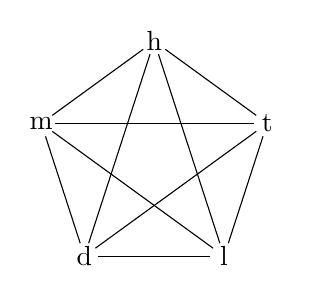
\begin{tikzpicture}[mystyle/.style={draw=white,shape=circle,fill=white}]	%Hebrew eodermdrome: הלמדת מה דלתה
\def\ngon{5}
\node[regular polygon,regular polygon sides=\ngon,minimum size=3cm] (p) {};
\foreach\x in {1,...,\ngon}{\node[mystyle] (p\x) at (p.corner \x){};}
\foreach\x in {1,...,\numexpr\ngon-1\relax}{
	\foreach\y in {\x,...,\ngon}{
		\draw (p\x) -- (p\y);}}

\node[circle,inner sep=0pt,fill=white] at (p1) {\cjRL{h}};	%ה
\node[circle,inner sep=0pt,fill=white] at (p5) {\cjRL{t}};	%ת
\node[circle,inner sep=0pt,fill=white] at (p4) {\cjRL{l}};	%ל
\node[circle,inner sep=0pt,fill=white] at (p3) {\cjRL{d}};	%ד
\node[circle,inner sep=0pt,fill=white] at (p2) {\cjRL{m}};	%מ
\end{tikzpicture}
%
%
\hspace{0.75cm}
%
%
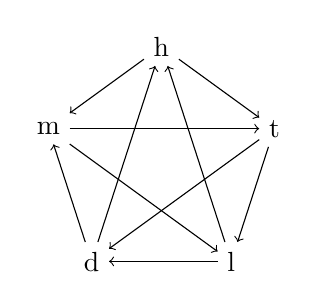
\begin{tikzpicture}	%Hebrew eodermdrome: הלמדת מה דלתה
\node[regular polygon,regular polygon sides=5,minimum width=30mm] (PG) {}
(PG.corner 1) node (PG1) {\cjRL{h}}		%ה
(PG.corner 5) node (PG2) {\cjRL{t}}		%ת
(PG.corner 4) node (PG3) {\cjRL{l}}		%ל
(PG.corner 3) node (PG4) {\cjRL{d}}		%ד
(PG.corner 2) node (PG5) {\cjRL{m}};	%מ

\foreach \S/\E in {
	1/2, 1/5,
	2/3, 2/4,
	3/1, 3/4,
	4/1, 4/5,
	5/2, 5/3%
} {\draw[->] (PG\S) -- (PG\E);}
\end{tikzpicture}
%
%
\hspace{0.75cm}
%
%
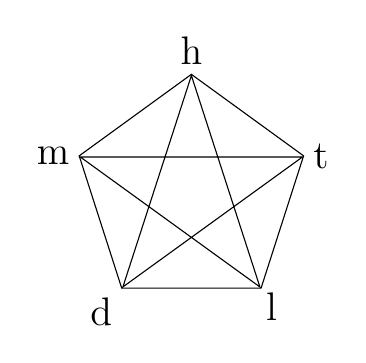
\begin{tikzpicture}[scale=1.5]	%Hebrew eodermdrome: הלמדת מה דלתה
%pentagon
\draw (0,0.69)--(-0.95,0)--(-0.59,-1.12)--(0.59,-1.12)--(0.95,0)--cycle;
%pentagram
\draw (-0.94,-0.01)--(0.94,-0.01)--(-0.58,-1.11)--(0,0.68)--(0.58,-1.11)--cycle;
%label nodes
\node [above] at (0,0.69) 			{\Large\cjRL{h}};		%ה
\node [right] at (0.95,0) 			{\Large\cjRL{t}};		%ת
\node [below right] at (0.55,-1.08) {\Large\cjRL{l}};		%ל
\node [below left] at (-0.59,-1.12) {\Large\cjRL{d}};		%ד
\node [left] at (-0.95,0) 			{\Large\cjRL{m}};		%מ
\end{tikzpicture}


\vspace{0.25cm}

\hspace{0.45cm}\cjRL{hlmdt mh dlth}

\hspace{-0.75cm}Did you learn what her door is?

%meaning: Did you learn what her door is?
\end{document}